\documentclass[11pt,a4paper,titlepage,leqno]{article}
\usepackage[utf8]{inputenc}
\usepackage{listings}
\usepackage{amsmath}
\usepackage{amsfonts}
\usepackage{amssymb}
\usepackage{makeidx}
\usepackage{graphicx}
\usepackage{color}
\usepackage{tikz-qtree}
\usepackage{float}

\title{Optimizacion de Consultas: Informe}
\author{Juan Pablo Civile \and Martin Sturla}
\date{18 de Septiembre de 2012}


\newcommand{\pr}[2]{\Pi_{#1}(#2)}
\newcommand{\join}[2]{#1 \bowtie #2}
\newcommand{\filter}[2]{\sigma_{#1}(#2)}
\newcommand{\ejercicio}[1]{
    \section*{Ejercicio #1}
    \setcounter{answer}{0}
}

\newcounter{answer}
\newcommand{\answer}{
    \addtocounter{answer}{1}
    \arabic{answer}.
}

\newcommand{\equ}[1]{
    \subsection*{\answer}
    \begin{equation}
        \tag*{}
        #1
    \end{equation}
}

\lstset{
    language = SQL,
    basicstyle=\footnotesize
}


\begin{document}

\maketitle

\ejercicio{1}

\equ{
    \pr{B, R.C, D}{
        \filter{R.A = 5}{
            \join{R}{S}
        }
    }
}

\equ{
    \pr{B, R.C, D}{
        \join{
            \filter{R.A = 5}{R}
        }{
            S
        }
    }
}

\equ{
    \join{
        \filter{A = 5}{
            \pr{A, C}{R}
        }
    }{
        \pr{S.C, D}{S}
    }
}

\ejercicio{2}

\begin{lstlisting}
    select Lista
    from R inner join S on R.b = S.b
    where cond
\end{lstlisting}

\ejercicio{3}

\equ{
    \pr{A, D}{
        \join{
            \filter{A = 10}{
                \pr{A, C}{R}
            }
        }{
            \pr{C, D}{
                \filter{E = 5}{S}
            }
        }
    }
}

\ejercicio{4}

\equ{
    \join{
        \filter{cond\_b \text{ AND } cond\_c}{R}
    }{
        \filter{cond\_d \text{ AND } cond\_c}{S}
    }
}

\equ{
    \filter{cond\_d \text{ OR } cond\_b}{
        \join{R}{S}
    }
}

\ejercicio{5}

\par Seg�n wikipedia, en el algebra relacional, el full outer join puede ser escrito como:

\begin{equation}
    R \times S = (R \ltimes S) \cup_{Set} (R \rtimes S)
    \label{eqn1}
\end{equation}

\par Donde:

\begin{itemize}
\item $\times$ es el outer join.
\item $\rtimes$ es left outer join.
\item $\ltimes$ es el operador right outer join.
\end{itemize}

\par Tambi�n se puede verificar, utilizando la misma fuente, que el left outer join es equivalente a (nota: utiliza un valor $\omega$ en vez de null):

\[
    R \rtimes S = (R \bowtie S) \cup ((R - \Pi_{r_1, r_2, ..., r_n}(R \bowtie S)) \otimes N)
\]

Donde $\bowtie$ es el natural join y $N$ representa NULL.

Combinando la primer ecuaci�n y que la selecci�n se puede distribuir en la uni�n, se llega a:


\[
    \sigma_{b<10}(R \times S) =  \sigma_{b<10}(R \ltimes S) \cup_{Set} \sigma_{b<10}(R \rtimes S)
\]

Distribuyendo nuevamente la selecci�n de una uni�n pero esta vez en la segunda ecuaci�n, se llega a:

\[
    \sigma_{b<10}(R \rtimes S) = \sigma_{b<10}(R \bowtie S) \cup \sigma_{b<10}((R - \Pi_{r_1, r_2, ..., r_n}(R \bowtie S)) \otimes N)
\]

Sin embargo, se verifica que $b$ es un atributo v�lido para tanto $R$ como $S$. Por lo tanto:
\[
\sigma_{b<10}(R \bowtie S) = \sigma_{b<10}(R) \bowtie \sigma_{b<10}(S)
\]

Prestando atenci�n al t�rmino de la resta, se puede verificar por equivalencia que se puede distribuir la selecci�n nuevamente. Por otro lado, 
como $b$ es en particular uno de los atributos de la lista, se puede intercambiar su �rden con la proyecci�n. Es decir:

\[
\sigma_{b<10}((R - \Pi_{r_1, r_2, ..., r_n}(R \bowtie S)) \otimes N) = \sigma_{b<10}(R) - \Pi_{r_1, r_2, ..., r_n}(\sigma_{b<10}(R \bowtie S)) \otimes N
\]

Si se distribuye la selecci�n en el natural join (es atributo de ambos), esta expresi�n se reduce a:

\[
\sigma_{b<10}(R \rtimes S) = (\sigma_{b<10}R \bowtie \sigma_{b<10}S) \cup  (\sigma_{b<10}(R) - \Pi_{r_1, r_2, ..., r_n}((\sigma_{b<10}R \bowtie \sigma_{b<10}S)) \otimes N)
\]

La demostraci�n para el right outer join es similar, con la excepci�n que el producto cartesiano es al rev�s, y los atributos en la lista son de la relaci�n 
$S$. Sin embargo, como $b$ pertenece a ambos, sigue siendo v�lida. Por lo tanto se llega a que:

\[
\sigma_{b<10}(R \ltimes S) =(\sigma_{b<10}R \bowtie \sigma_{b<10}S) \cup  N \otimes (\sigma_{b<10}(S) -  \Pi_{s_1, s_2, ..., s_n}((\sigma_{b<10}R \bowtie \sigma_{b<10}S)))
\]

Por lo cual el outer join es equivalente a la uni�n de estas �ltimas dos ecuaciones. 

Sea $T= \sigma_{b<10}R$ y $Q=\sigma_{b<10}S$. Entonces:

\begin{eqnarray}
    \nonumber \sigma_{b<10}(R \times S) & = & ( T\bowtie Q) \cup (T - \Pi_{r_1, r_2, \dots, r_n}(T \bowtie Q) \otimes N) \\
    \nonumber  & & \cup_{Set} \\
    \nonumber  & & (T \bowtie Q) \cup N \otimes (Q - \Pi_{s_1, s_2, \dots, s_n}(T \bowtie q)) \\
    \nonumber & = & (\sigma_{b<10}(R)) \times (\sigma_{b<10}(S))
\end{eqnarray}

\ejercicio{6}

\equ{
    \frac{ \#W }{ Card(W, a) * Card(W, b) } = \frac{ 100 }{ 800 } = \frac{1}{8}
}

\equ{
    \frac{
        \#W * \#X * \#Z
    }{
        max(Card(W, b), Card(X, b)) * max(Card(X, c), Card(Z, c))
    }
    = 200
}

\ejercicio{7}

\equ{
    \frac{
        \#S * \#T
    }{
        Card(S, b) * max(Card(S, c), Card(T, c))
    }
    = 48
}

\equ{
    \text{Costo de } \join{R}{S} =
    \frac{
        \#R * \#S
    }{
        max(Card(R, b), Card(S, b))
    }
    = 600
}

No se puede decir nada del factor de selectividad $R.A < S.C$, dado que no son constantes. Se requiere usar un histograma.

\ejercicio{8}

\subsection*{\answer}

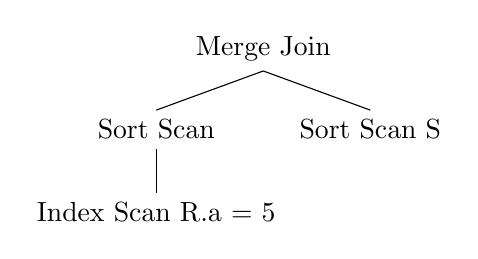
\begin{tikzpicture}
    \Tree [. {Merge Join}
        [. {Sort Scan} {Index Scan R.a = 5} ]
        [. {Sort Scan S} ]
    ]
\end{tikzpicture}

\subsection*{\answer}

No usa indice


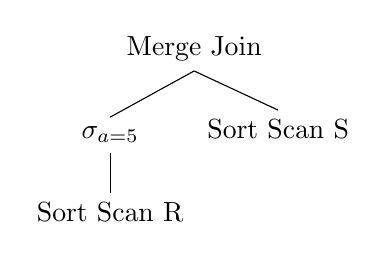
\begin{tikzpicture}
    \Tree [. {Merge Join}
        [. {$\sigma_{a = 5}$} {Sort Scan R} ]
        [. {Sort Scan S} ]
    ]
\end{tikzpicture}

\subsection*{\answer}

No prioriza seleccion, ni hace uso de indice.


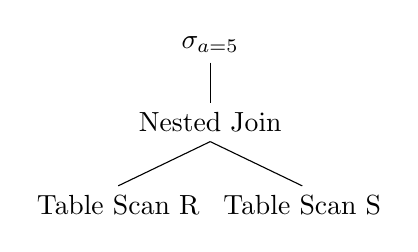
\begin{tikzpicture}
    \Tree [. {$\sigma_{a = 5}$}
        [. {Nested Join}
            [. {Table Scan R} ]
            [. {Table Scan S} ]
        ]
    ]
\end{tikzpicture}

\subsection*{\answer}

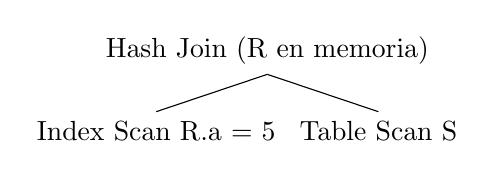
\begin{tikzpicture}
    \Tree [. {Hash Join (R en memoria)}
        [. {Index Scan R.a = 5} ]
        [. {Table Scan S} ]
    ]
\end{tikzpicture}

\ejercicio{9}

\subsection*{\answer}

\paragraph{Plan 1}
\begin{equation}
    \tag*{}
    B(R) + \frac{ \#R * \#S }{ Card(S, b) } = 10001000
\end{equation}

\paragraph{Plan 2}
\begin{equation}
    \tag*{}
    B(R) + \frac{\#R * B(S)}{Card(S,c)} = 2501000
\end{equation}

\subsection*{\answer}

Hacer uso de un Table Based Nested Join da un mejor resultado, dado que los bloques de R contienen muchas tuplas.

\begin{equation}
    \tag*{}
    B(R) * B(S) = 1000000
\end{equation}

\ejercicio{10}

El sort usara aproximadamente $n log_{10}(n)$ accesos a bloques de R: $B(R) log_{10}(B(R)) = 3 * 10^3$.

Para ordenar S por C usara \texttt{IC}, que es clustered, con costo $B(S)$. Luego hara un two-way sort. El merge costara lo mismo que leer ambas listas ordenadas.

Por lo tanto, el total sera $3 * 10^3 + (10^3 + 10^3) = 5 * 10^3$.

\ejercicio{11}

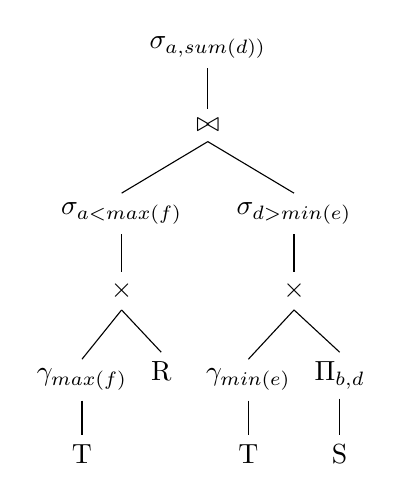
\begin{tikzpicture}
    \Tree [. {$\sigma_{a, sum(d))}$} 
        [. {$\bowtie$}
            [. {$\sigma_{a < max(f)}$}
                [. {$\times$}
                    [. {$\gamma_{max(f)}$} {T} ]
                    [. {R} ]
                ]
            ]
            [. {$\sigma_{d > min(e)}$} 
                [. {$\times$}
                    [. {$\gamma_{min(e)}$} {T} ]
                    [. {$\Pi_{b, d}$} {S} ]
                ]
            ]
        ]
    ]
\end{tikzpicture}

\end{document}
